\chapter{Eksamen}
\subsection*{Prøveform, tilrettelæggelse og formkrav}
Prøven er individuel og består af en individuel videopræsentation af en selvvalgt case med anvendelse af relevante teorier og værktøjer inden for IoT. Videoen skal have en varighed af ca. 5 minutter.

\subsection*{Forudsætninger for at deltage i prøven}
For at deltage i prøven skal indholdet i videopræsentationen være redeligt. Det skal desuden opfylde formkrav samt være korrekt og rettidigt afleveret jf. årsplan på Campus.
\newline\newline\noindent
Det er et forudsætningskrav for at deltage i prøven, at man via underskrift bekræfter, at man er ansvarlig for udarbejdelsen af videopræsentationen. Dette sker rent praktisk ved upload i WISEflow.
\newline\newline\noindent
Manglende opfyldelse af blot en eller flere forudsætninger betyder, at den studerende ikke kan deltage i prøven, og der er brugt et prøveforsøg.

\subsection*{Bedømmelseskriterier og censurtype}
Bedømmelseskriterierne for valgfagets prøve er lig med læringsmål for valgfaget. Bedømmelse sker efter 7-trinsskalaen, og der er intern censur. Der gives en samlet karakter ud fra en helhedsvurdering. I bedømmelsen indgår videopræsentationen.

\subsection*{Anvendelse af hjælpemidler}
Under prøverne er anvendelse af hjælpemidler, herunder elektroniske hjælpemidler, tilladt, medmindre der i bekendtgørelsen eller studieordningen for den enkelte uddannelse er fastsat begrænsninger i anvendelsen.
\newline\newline\noindent
Eventuelle regler for indskrænkning af brug for hjælpemidler vil fremgå af beskrivelsen af den enkelte prøve.

\section{Teknologikæde}
\subsubsection*{IoT Projekt med ESP32}
Internet of Things (IoT) er en teknologi, der forbinder forskellige enheder til internettet og med hinanden. I dette afsnit vil vi undersøge en komplet IoT-løsning ved hjælp af ESP32, en populær mikrocontroller med indbygget Wi-Fi og Bluetooth, og gennemgå hele teknologikæden fra sensorer til integration med andre systemer.

\subsection*{Sensorer og Aktuatorer}
Vi kan tilslutte en DHT22 temperatur- og fugtighedssensor til ESP32'en. Denne sensor vil opsamle realtidsdata om temperatur og fugtighed.

\subsection*{Embedded Systems og Mikrocontrollere}
ESP32'en læser data fra DHT22-sensoren og behandler dem. Den kan udføre en simpel analyse som at bestemme, om temperaturen er over et bestemt niveau.

\subsection*{Kommunikation}
ESP32'en kan konfigureres til at sende disse data over Wi-Fi ved hjælp af MQTT-protokollen til en MQTT-broker. Denne broker kan være en lokal server eller en cloud-baseret service.

\subsection*{Datacenter og Cloud Computing}
MQTT-brokeren modtager data og lagrer dem i en database. Dette kan være en SQL-database, der kører på en server i et datacenter eller i skyen (f.eks., AWS, Azure, Firebase).

\subsection*{Analyser og Applikationer}
Data fra databasen kan analyseres yderligere ved hjælp af et dataanalyseværktøj som Python med Pandas. Du kan bygge en webapplikation med en teknologi som Node.js for at præsentere data til brugerne.

\subsection*{Sikkerhed}
Hele systemet skal sikres for at forhindre uautoriseret adgang og manipulation. Dette inkluderer at bruge stærke adgangskoder, opdateret firmware/software, og sikkerhedsprotokoller som TLS til krypteret dataoverførsel.

\subsection*{Integration med andre systemer}
Denne IoT-løsning kan integreres med et smart hjem system. Hvis temperaturen overstiger et bestemt niveau, kan systemet automatisk tænde en ventilator ved at sende et signal til en smart stikkontakt.

\subsection{Samlet Flow}
Dette eksempel illustrerer, hvordan en ESP32 kan bruges til at skabe en komplet IoT-løsning, der strækker sig fra den fysiske sensor til en slutbrugerapplikation, med fuld overvejelse af kommunikation, databehandling, analyse, sikkerhed og integration. Det viser, hvordan forskellige teknologier og protokoller kan samarbejde om at skabe en sammenhængende og nyttig løsning.
\newline\newline\noindent
Teknologikæden er repræsenteret i nedenstående figur fra sensor til den applikation, som brugeren anvender.
%\begin{figure}[!h]
%	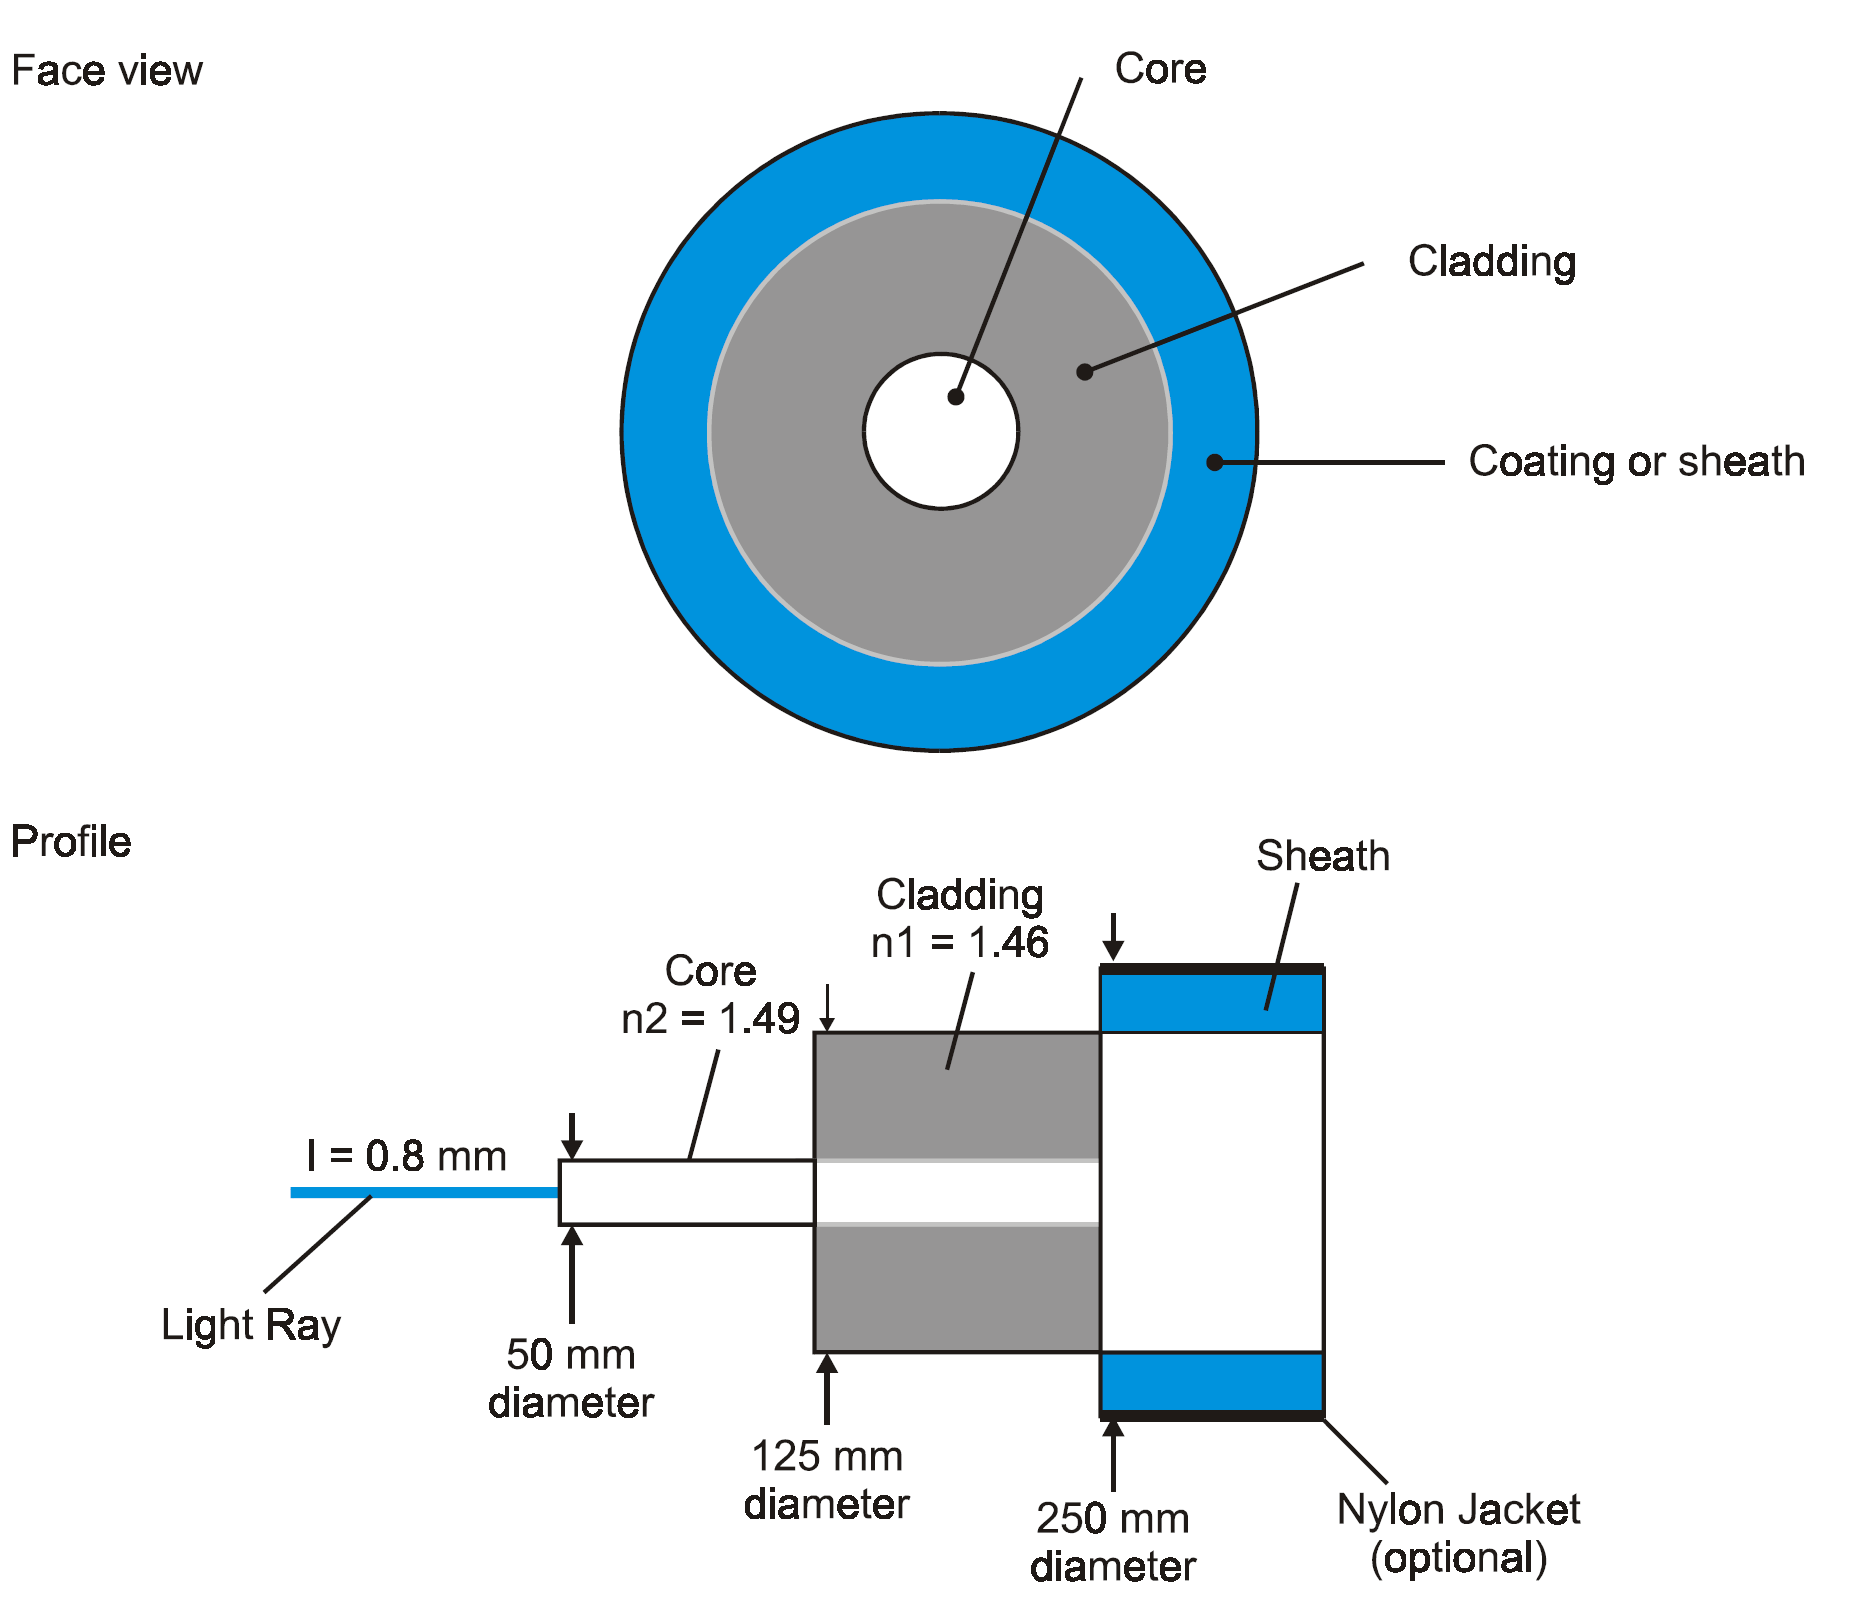
\includegraphics[width=\textwidth]{fig/fig35.png}	
%\end{figure}


\chapter{Projektbeskrivelse for Eksamensprojekt: IoT Smart House}
\section*{Formål}
Formålet med dette eksamensprojekt er at udvikle et IoT Smart House, hvor der redegøres for teknologikæden og anvendt IoT-teknologi. Projektet vil inkludere implementering og integration af forskellige sensorer og aktuatorer, kommunikationsprotokoller, datalagring, og et kontrolpanel ved hjælp af Node-RED. Projektet skal demonstreres i en 5-minutters videopræsentation, hvor løsningen beskrives og evalueres.

\section*{Projektindhold}

\subsection*{Teknologikæde}
Dette projekt vil udforske en komplet teknologikæde, der begynder med sensorer og aktuatorer forbundet til en ESP32-mikrocontroller. Data fra sensorerne vil blive behandlet og sendt videre ved hjælp af en eller flere kommunikationsprotokoller. Disse data vil blive lagret i en database, som f.eks. Firebase Realtime Database (RTDB), og præsenteret i et dashboard udviklet i Node-RED. Projektet vil også undersøge sikkerhedsaspekter af IoT-løsningen.

\subsection*{Anvendt IoT-teknologi}

\paragraph{Node-RED og Dashboard}
Node-RED vil blive brugt som et kontrolpanel til at overvåge og styre IoT-enhederne. Et brugervenligt dashboard vil blive udviklet for at visualisere data fra sensorer og give kontrol over aktuatorer.

\paragraph{Kommunikationsprotokoller}
To til tre kommunikationsprotokoller vil blive implementeret for at forbinde enhederne i Smart House. Eksempler kan være MQTT, HTTP, og Modbus, som vil blive anvendt til at overføre data mellem ESP32 og centrale systemer.

\paragraph{Data Lagring}
Data fra sensorerne vil blive sendt til en Firebase Realtime Database (RTDB), hvor de lagres for senere analyse og overvågning. Alternativt kan en anden database anvendes, afhængigt af projektets krav.

\subsection*{Prøveform og Præsentation}
Projektet vil blive præsenteret gennem en individuel videopræsentation, hvor de valgte teknologier og løsninger forklares og demonstreres. Videoen skal være ca. 5 minutter lang og skal tydeligt vise forståelsen af IoT-teknologi og dens anvendelse i et Smart House.

\subsection*{Opsummering}
Dette eksamensprojekt har til formål at udvikle og demonstrere en IoT-baseret Smart House-løsning, der integrerer flere teknologier, herunder Node-RED, kommunikationsprotokoller og datalagring. Projektet vil blive præsenteret i en videopræsentation, som viser de praktiske anvendelser af IoT i et moderne hjem.

\subsection*{Sensor \& aktuator}
IoT Smart House har et antal sensor og aktuatorer som er følgende:
\begin{itemize}
	\item DHT11 - Temperatur- og fugtighedssensor (tilsluttet IO17).
	\item PIR Motion Sensor - Bevægelsessensor (tilsluttet IO14).
	\item Gas Sensor - (tilsluttet IO23).
	\item Steam Sensor - (tilsluttet IO34).
	\item RFID Module - (tilsluttet via I2C).
	\item LED Module - Yellow LED (tilsluttet IO12).
	\item 6812RGB LED - RGB LED (tilsluttet IO26).
	\item Buzzer - (tilsluttet IO25).
	\item Servo Motor (Windows) - Styring af vinduer (tilsluttet IO5).
	\item Servo Motor (Doors) - Styring af døre (tilsluttet IO13).
	\item Left Button Module - Venstre knap (tilsluttet IO16).
	\item Right Button Module - Højre knap (tilsluttet IO27).
	\item Fan - (tilsluttet IO18 og IO19).
	\item LCD1602 Display - Tilsluttet via I2C.
\end{itemize}

\clearpage

\subsection*{Sensor \& aktuator kode}
\subsubsection*{DHT11 - Temperatur- og fugtighedssensor}
\begin{lstlisting}[language=C++]
	#include <DHT.h>
	
	// Define the DHTSensor class directly in the .ino file
	class DHTSensor {
		private:
		uint8_t pin;  // Pin number where the sensor is connected
		DHT dht;      // DHT object for handling the sensor
		
		public:
		// Constructor to initialize the DHTSensor with a pin and sensor type (DHT11/DHT22)
		DHTSensor(uint8_t p, uint8_t type) : pin(p), dht(p, type) {}
		
		// Method to initialize the sensor
		void begin() {
			dht.begin();
		}
		
		// Method to read temperature from the sensor
		float readTemperature() {
			float temp = dht.readTemperature();
			if (isnan(temp)) {
				Serial.println("Failed to read temperature!");
				return -1.0;
			}
			return temp;
		}
		
		// Method to read humidity from the sensor
		float readHumidity() {
			float humidity = dht.readHumidity();
			if (isnan(humidity)) {
				Serial.println("Failed to read humidity!");
				return -1.0;
			}
			return humidity;
		}
	};
	
	// Create an object of the DHTSensor class
	DHTSensor dhtSensor(17, DHT11);
	
	void setup() {
		Serial.begin(115200);   // Initialize serial communication at 115200 baud rate
		dhtSensor.begin();      // Initialize the DHT sensor
	}
	
	void loop() {
		// Read temperature and humidity from the sensor
		float temperature = dhtSensor.readTemperature();
		float humidity = dhtSensor.readHumidity();
		
		// Print temperature if it's valid
		if (temperature != -1.0) {
			Serial.print("Temperature: ");
			Serial.print(temperature);
			Serial.println(" C");
		}
		
		// Print humidity if it's valid
		if (humidity != -1.0) {
			Serial.print("Humidity: ");
			Serial.print(humidity);
			Serial.println(" %");
		}
		
		delay(2000);  // Wait 2 seconds between readings
	}
\end{lstlisting}
\clearpage
\subsubsection*{PIR Motion Sensor}
\begin{lstlisting}[language=C++]
	// Define the PIRSensor class directly in the .ino file
	class PIRSensor {
		private:
		uint8_t pin;  // Pin number where the PIR sensor is connected
		
		public:
		// Constructor to initialize the PIRSensor with a specific pin
		PIRSensor(uint8_t p) : pin(p) {
			pinMode(pin, INPUT);  // Set the PIR sensor pin as input
		}
		
		// Method to check if motion is detected by the PIR sensor
		bool isMotionDetected() {
			return digitalRead(pin) == HIGH;  // Return true if motion is detected
		}
	};
	
	// Create an object of the PIRSensor class
	PIRSensor pirSensor(14);
	
	void setup() {
		Serial.begin(115200);  // Initialize serial communication at 115200 baud rate
	}
	
	void loop() {
		// Check if motion is detected by the PIR sensor
		if (pirSensor.isMotionDetected()) {
			Serial.println("Motion detected!");  // Print a message if motion is detected
		} else {
			Serial.println("No motion.");  // Print a message if no motion is detected
		}
		
		delay(2000);  // Wait 2 seconds between checks
	}
\end{lstlisting}
\clearpage
\subsubsection*{Gas Sensor}
\begin{lstlisting}[language=C++]
	// Define the GasSensor class directly in the .ino file
	class GasSensor {
		private:
		uint8_t pin;  // Pin number where the Gas sensor is connected
		
		public:
		// Constructor to initialize the GasSensor with a specific pin
		GasSensor(uint8_t p) : pin(p) {
			pinMode(pin, INPUT);  // Set the Gas sensor pin as input
		}
		
		// Method to read the gas level from the sensor
		int readGasLevel() {
			return analogRead(pin);  // Return the analog value from the sensor
		}
	};
	
	// Create an object of the GasSensor class
	GasSensor gasSensor(23);
	
	void setup() {
		Serial.begin(115200);  // Initialize serial communication at 115200 baud rate
	}
	
	void loop() {
		// Read the gas level from the sensor
		int gasLevel = gasSensor.readGasLevel();
		Serial.print("Gas level: ");
		Serial.println(gasLevel);
		
		delay(2000);  // Wait 2 seconds between readings
	}
\end{lstlisting}
\clearpage	
\subsubsection*{Steam Sensor}
\begin{lstlisting}[language=C++]
	// Define the SteamSensor class directly in the .ino file
	class SteamSensor {
		private:
		uint8_t pin;  // Pin number where the Steam sensor is connected
		
		public:
		// Constructor to initialize the SteamSensor with a specific pin
		SteamSensor(uint8_t p) : pin(p) {
			pinMode(pin, INPUT);  // Set the Steam sensor pin as input
		}
		
		// Method to read the steam level from the sensor
		int readSteamLevel() {
			return analogRead(pin);  // Return the analog value from the sensor
		}
	};
	
	// Create an object of the SteamSensor class
	SteamSensor steamSensor(34);
	
	void setup() {
		Serial.begin(115200);  // Initialize serial communication at 115200 baud rate
	}
	
	void loop() {
		// Read the steam level from the sensor
		int steamLevel = steamSensor.readSteamLevel();
		Serial.print("Steam level: ");
		Serial.println(steamLevel);
		
		delay(2000);  // Wait 2 seconds between readings
	}
\end{lstlisting}
\clearpage
\subsubsection*{RFID Module}
\begin{lstlisting}[language=C++]
	#include <Wire.h>
	#include <MFRC522_I2C.h>
	
	// Define the RFIDModule class directly in the .ino file
	class RFIDModule {
		private:
		uint8_t address;  // I2C address for the RFID module
		MFRC522 mfrc522;
		
		public:
		// Constructor to initialize the RFIDModule with a specific I2C address
		RFIDModule(uint8_t addr) : address(addr), mfrc522(addr) {}
		
		// Method to initialize the RFID module
		void begin() {
			mfrc522.PCD_Init();
		}
		
		// Method to check if a new card is present and read its UID
		bool readCardUID() {
			if (!mfrc522.PICC_IsNewCardPresent() || ! mfrc522.PICC_ReadCardSerial()) {
				return false;
			}
			
			Serial.print("Card UID:");
			for (byte i = 0; i < mfrc522.uid.size; i++) {
				Serial.print(mfrc522.uid.uidByte[i] < 0x10 ? " 0" : " ");
				Serial.print(mfrc522.uid.uidByte[i], HEX);
			}
			Serial.println();
			return true;
		}
	};
	
	// Create an object of the RFIDModule class
	RFIDModule rfidModule(0x28);  // I2C address for the RFID module
	
	void setup() {
		Serial.begin(115200);  // Initialize serial communication at 115200 baud rate
		Wire.begin();          // Initialize I2C communication
		rfidModule.begin();    // Initialize RFID module
	}
	
	void loop() {
		// Check if a card is present and read its UID
		if (rfidModule.readCardUID()) {
			Serial.println("Card detected.");
		} else {
			Serial.println("No card detected.");
		}
		
		delay(1000);  // Wait 1 second between checks
	}
\end{lstlisting}
\clearpage
\subsubsection*{LED Module - Yellow LED}
\begin{lstlisting}[language=C++]
	// Define the LEDModule class directly in the .ino file
	class LEDModule {
		private:
		uint8_t pin;  // Pin number where the LED is connected
		
		public:
		// Constructor to initialize the LEDModule with a specific pin
		LEDModule(uint8_t p) : pin(p) {
			pinMode(pin, OUTPUT);  // Set the LED pin as output
		}
		
		// Method to turn on the LED
		void turnOn() {
			digitalWrite(pin, HIGH);  // Set the pin high to turn on the LED
		}
		
		// Method to turn off the LED
		void turnOff() {
			digitalWrite(pin, LOW);  // Set the pin low to turn off the LED
		}
	};
	
	// Create an object of the LEDModule class
	LEDModule yellowLED(12);
	
	void setup() {
		Serial.begin(115200);  // Initialize serial communication at 115200 baud rate
	}
	
	void loop() {
		// Turn the LED on and off with a 1-second delay
		yellowLED.turnOn();
		Serial.println("Yellow LED is ON");
		delay(1000);
		
		yellowLED.turnOff();
		Serial.println("Yellow LED is OFF");
		delay(1000);
	}
\end{lstlisting}
\clearpage
\subsubsection*{Buzzer}
\begin{lstlisting}[language=C++]
	// Define the Buzzer class directly in the .ino file
	class Buzzer {
		private:
		uint8_t pin;  // Pin number where the Buzzer is connected
		
		public:
		// Constructor to initialize the Buzzer with a specific pin
		Buzzer(uint8_t p) : pin(p) {
			pinMode(pin, OUTPUT);  // Set the Buzzer pin as output
		}
		
		// Method to turn on the Buzzer
		void turnOn() {
			digitalWrite(pin, HIGH);  // Set the pin high to turn on the Buzzer
		}
		
		// Method to turn off the Buzzer
		void turnOff() {
			digitalWrite(pin, LOW);  // Set the pin low to turn off the Buzzer
		}
		
		// Method to make the Buzzer beep for a specified duration
		void beep(unsigned int duration) {
			turnOn();
			delay(duration);
			turnOff();
		}
	};
	
	// Create an object of the Buzzer class
	Buzzer buzzer(25);
	
	void setup() {
		Serial.begin(115200);  // Initialize serial communication at 115200 baud rate
	}
	
	void loop() {
		// Make the Buzzer beep with a 500ms duration
		buzzer.beep(500);
		Serial.println("Buzzer beeped");
		delay(2000);  // Wait 2 seconds between beeps
	}
\end{lstlisting}
\clearpage
\subsubsection*{Servo Motor}
Efersom servo motor er den samme kode for både dør og vindue så laves kun en klasse, men fordi det er en klasse så kan koden genbruges.
\begin{lstlisting}[language=C++]
	#include <ESP32Servo.h>
	
	// Define the ServoMotor class directly in the .ino file
	class ServoMotor {
		private:
		Servo servo;       // Servo object
		uint8_t pin;       // Pin number where the servo is connected
		int position;      // Current position of the servo
		
		public:
		// Constructor to initialize the ServoMotor with a specific pin
		ServoMotor(uint8_t p) : pin(p), position(0) {}
		
		// Method to attach the servo to the specified pin
		void begin() {
			servo.attach(pin);
		}
		
		// Method to set the position of the servo within the range 0-180 degrees
		void setPosition(int pos) {
			if (pos >= 0 && pos <= 180) {
				position = pos;
				servo.write(position);  // Move servo to the specified position
				Serial.print("Servo moved to: ");
				Serial.print(position);
				Serial.println(" degrees");
			} else {
				Serial.println("Error: Position out of range (0-180)");
			}
		}
		
		// Method to get the current position of the servo
		int getPosition() {
			return position;
		}
	};
	
	// Create an object of the ServoMotor class
	ServoMotor myServo(5);
	
	void setup() {
		Serial.begin(115200);  // Initialize serial communication at 115200 baud rate
		myServo.begin();       // Attach the servo motor
		myServo.setPosition(90);  // Start with the servo at 90 degrees
	}
	
	void loop() {
		// Example of setting the servo to different angles
		delay(2000);
		myServo.setPosition(45);  // Move the servo to 45 degrees
		delay(2000);
		myServo.setPosition(135); // Move 
	\end{lstlisting}
	\clearpage
	\subsubsection*{Button Module}
	Efersom servo motor er den samme kode for både dør og vindue så laves kun en klasse, men fordi det er en klasse så kan koden genbruges.
	\begin{lstlisting}[language=C++]
		#include <Arduino.h>
		
		volatile bool buttonStateChanged = false;  // Flag to indicate button state change
		
		class ButtonModule {
			private:
			uint8_t pin;  // Pin number where the button is connected
			int buttonState;  // Variable to store the current state of the button
			
			public:
			// Constructor to initialize the ButtonModule with a specific pin
			ButtonModule(uint8_t p) : pin(p), buttonState(HIGH) {
				pinMode(pin, INPUT_PULLUP);  // Set the button pin as input with internal pull-up
				attachInterrupt(digitalPinToInterrupt(pin), handleInterrupt, CHANGE);  // Attach interrupt to handle button state change
			}
			
			// Method to check if the button state changed
			int getState() {
				if (buttonStateChanged) {
					buttonStateChanged = false;  // Reset the flag after reading
					buttonState = digitalRead(pin);  // Read and return the current state of the button
				}
				return buttonState;  // Return the last known state if no change
			}
			
			// Interrupt Service Routine to handle the button state change
			static void handleInterrupt() {
				buttonStateChanged = true;  // Set the flag to indicate button state change
			}
		};
		
		// Create an object of the ButtonModule class
		ButtonModule button(16);  // Replace 16 with the actual pin number if necessary
		
		void setup() {
			Serial.begin(115200);  // Initialize serial communication at 115200 baud rate
		}
		
		void loop() {
			// Check if the button state changed and print the result
			int buttonState = button.getState();
			Serial.print("Button state: ");
			Serial.println(buttonState == LOW ? "Pressed" : "Released");
			
			delay(100);  // Small delay for debounce
		}
	\end{lstlisting}
	\clearpage
	\subsubsection*{Fan}
	\begin{lstlisting}[language=C++]
		#include <Arduino.h>
		
		class Fan {
			private:
			uint8_t pinIn1;  // Pin number for IN1 on the fan driver
			uint8_t pinIn2;  // Pin number for IN2 on the fan driver
			
			public:
			// Constructor to initialize the Fan with specific pins
			Fan(uint8_t in1, uint8_t in2) : pinIn1(in1), pinIn2(in2) {
				pinMode(pinIn1, OUTPUT);  // Set pinIn1 as output
				pinMode(pinIn2, OUTPUT);  // Set pinIn2 as output
				control(LOW);             // Ensure the fan is off at the start
			}
			
			// Method to control the fan with HIGH or LOW
			void control(int state) {
				if (state == HIGH) {
					digitalWrite(pinIn1, HIGH);  // Set IN1 high
					digitalWrite(pinIn2, LOW);   // Set IN2 low
					Serial.println("Fan is ON");
				} else {
					digitalWrite(pinIn1, LOW);   // Set IN1 low
					digitalWrite(pinIn2, LOW);   // Set IN2 low
					Serial.println("Fan is OFF");
				}
			}
		};
		
		// Create an object of the Fan class
		Fan fan(18, 19);  // Replace 18 and 19 with the actual pin numbers if necessary
		
		void setup() {
			Serial.begin(115200);  // Initialize serial communication at 115200 baud rate
			fan.control(LOW);      // Start with the fan off
		}
		
		void loop() {
			delay(2000);
			fan.control(HIGH);  // Turn the fan on
			delay(2000);
			fan.control(LOW);   // Turn the fan off
		}
	\end{lstlisting}
	
	\subsubsection*{LCD1602 Display}
	\begin{lstlisting}[language=C++]
		#include <Wire.h>
		#include <LiquidCrystal_I2C.h>
		
		class LCD1602Display {
			private:
			LiquidCrystal_I2C lcd;  // LCD object
			
			public:
			// Constructor to initialize the LCD with the I2C address
			LCD1602Display(uint8_t lcdAddr) : lcd(lcdAddr, 16, 2) {
				lcd.init();  // Initialize the LCD
				lcd.backlight();  // Turn on the backlight
			}
			
			// Method to print text on the first row
			void printLine1(const char* row1) {
				lcd.setCursor(0, 0);  // Set cursor to the first row, first column
				lcd.print("                "); // Clear the line
				lcd.setCursor(0, 0);  // Set cursor back to the first row
				lcd.print(row1);  // Print text on the first row
			}
			
			// Method to print text on the second row
			void printLine2(const char* row2) {
				lcd.setCursor(0, 1);  // Set cursor to the second row, first column
				lcd.print("                "); // Clear the line
				lcd.setCursor(0, 1);  // Set cursor back to the second row
				lcd.print(row2);  // Print text on the second row
			}
		};
		
		// Create an object of the LCD1602Display class with I2C address 0x27
		LCD1602Display lcdDisplay(0x27);
		
		void setup() {
			// Initial text on the LCD
			lcdDisplay.printLine1("Hello, World!");
			lcdDisplay.printLine2("Welcome!");
		}
		
		void loop() {
			// Example: Change text on the LCD every 5 seconds
			delay(5000);
			lcdDisplay.printLine1("Line 1 Updated");
			lcdDisplay.printLine2("Line 2 Updated");
			
			delay(5000);
			lcdDisplay.printLine1("Another Line 1");
			lcdDisplay.printLine2("Another Line 2");
		}
	\end{lstlisting}
	
	\subsection*{Alt kode}
	\begin{lstlisting}
		
	\end{lstlisting}